\section{SOLID implementatie}
Tijdens het realiseren zijn de ontwerpprincipes van SOLID (zie \ref{subsecion:SoftwareArhitectuur} voor meer informatie) meegenomen.
In deze sectie wordt er meer ingezoomd naar de implementatie van de SOLID principes en hoe dat tot uiting is gekomen.

\whitespace
De softwarearchitectuur maakt gebruik van handlers.
Een handler is een encapsulatie van de business logica voor een bepaalde context.
Deze handler heeft maar één taak waardoor het aan het \textit{Single-responsibility principle} voldoet.
In het voorbeeld (figuur \ref{fig:ImplementationUpsertItemHandler}) is te zien dat deze handlers als taak heeft het upserten van Items.
Upserten is het principe van het \textit{updaten} van de entiteit als hij bestaat en als dat niet het geval is het \textit{insert}.
In figuur \ref{fig:interfaceUpsertItemHandler} is te zien dat hij 2 methodes heeft, maar beide methodes hebben dezelfde \qw{taak}, het upserten van items.

\whitespace
\begin{graphic}
    \captionsetup{type=figure}
    \caption{UpsertItemHandler Implementatie}
    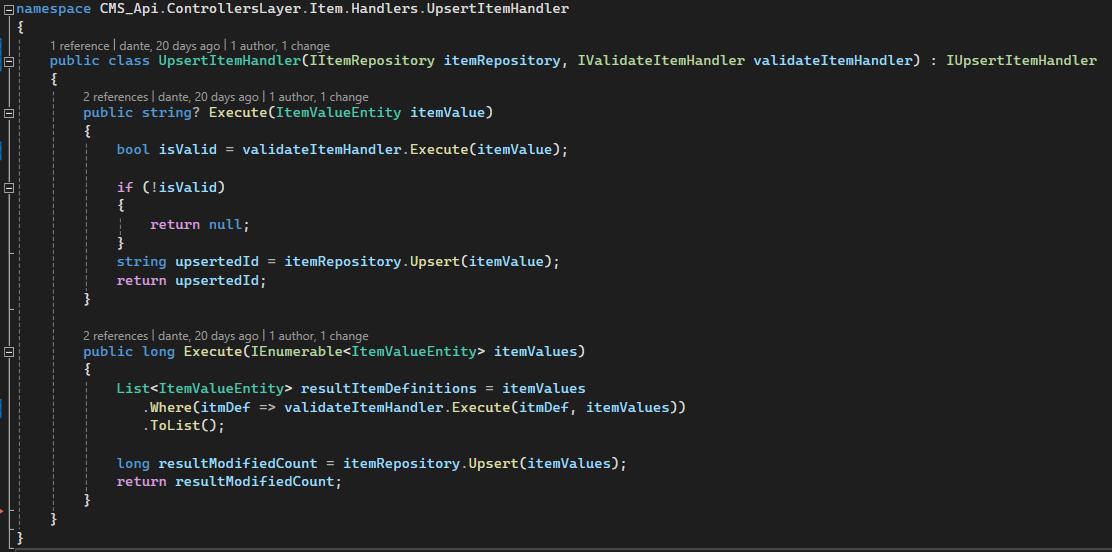
\includegraphics[scale=0.5]{ImplementationUpsertItemHandler.png}
    \label{fig:ImplementationUpsertItemHandler}
\end{graphic}

\whitespace[2]
\begin{graphic}
    \captionsetup{type=figure}
    \caption{UpsertItemHandler interface}
    \includegraphics[scale=0.6]{interfaceUpsertItemHandler.png}
    \label{fig:interfaceUpsertItemHandler}
\end{graphic}

\whitespace
In de verschillende handlers wordt er gebruikgemaakt van het \textit{Open\slash Closed principle}.
Doordat de handler gebruik maakt van de interface \textit{IUpsertItemHandler} zou er makkelijk een nieuwe implementatie toegevoegd kunnen worden.
Omdat de handlers maar één taak hebben blijft hun interface erg klein (meestal 1 of 2 methoden).
Dit zorgt dat de interfaces erg gefocust blijven op hun taak en er daarmee voldaan wordt aan het \textit{Interface segrigation principle}.
De injectie van de concrete implementatie wordt gedaan door middel van \textit{Dependency injection}.
Door gebruik te maken van \textit{depencency injection} wordt er ook voldaan aan het \textit{Depencency inversion principle}.

\subsection{Repository pattern}
Om de data laag en de logica van elkaar te scheiden is er gebruikt van een repository pattern \parencite{RepositoryPattern}.
Het repository pattern is een structureel design pattern dat de data laag en logica van de applicatie scheidt.
Dit wordt bereikt door middel van een abstracte tussenlaag die communicatie verzorgt tussen de logica en de data laag.

\whitespace
Dit leidt tot een scheiding tussen de logica en de data, waardoor voldaan wordt aan het \textit{single responsibility principle}.
Dit resulteert in beter testbare code, wat de betrouwbaarheid van het programma verhoogt.
Bovendien voorkomt dit dat de codebase afhankelijk is van één specifieke databaseprovider.

\whitespace
Dit is geïmplementeerd door de logica af te laten hangen van een interface in plaats van een concrete implementatie.
Vervolgens wordt bij initialisatie van de applicatie  een concrete versie geïnjecteerd.
Een visualisatie van de geïmplementeerde versie is te zien in figuur \ref{fig:RepositoryPattern}.
In figuur \ref{fig:RepositoryPattern} is te zin dat de verschillende handlers gebruik maken van de interface van de repository.
Hierdoor zou er in de toekomst een ander concrete implementatie geïnjecteerd kunnen worden zonder de correctheid van het programma te veranderen.
Er is ook een klassen diagram gemaakt van de implementatie die is te vinden in \ref{fig:RepositoryPatternUML}.


\whitespace[2]
\begin{graphic}
    \captionsetup{type=figure}
    \caption{Repository pattern implementatie}
    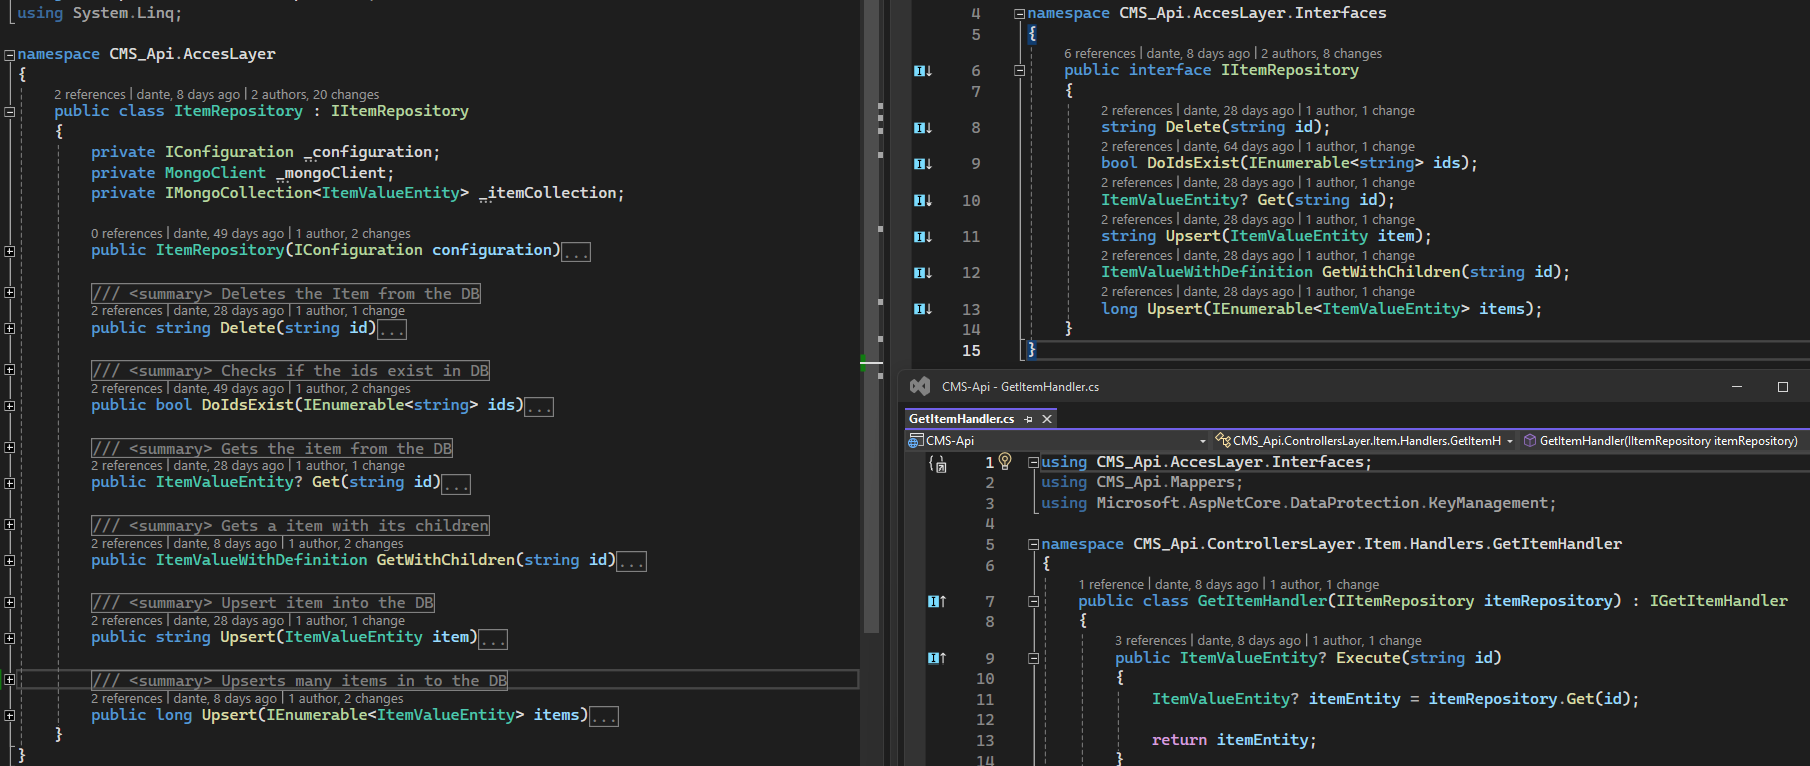
\includegraphics[scale=0.32]{ImplementationRepositoryPattern.png}
    \label{fig:RepositoryPattern}
\end{graphic}

\begin{graphic}
    \captionsetup{type=figure}
    \caption{Repository pattern implementatie UML}
    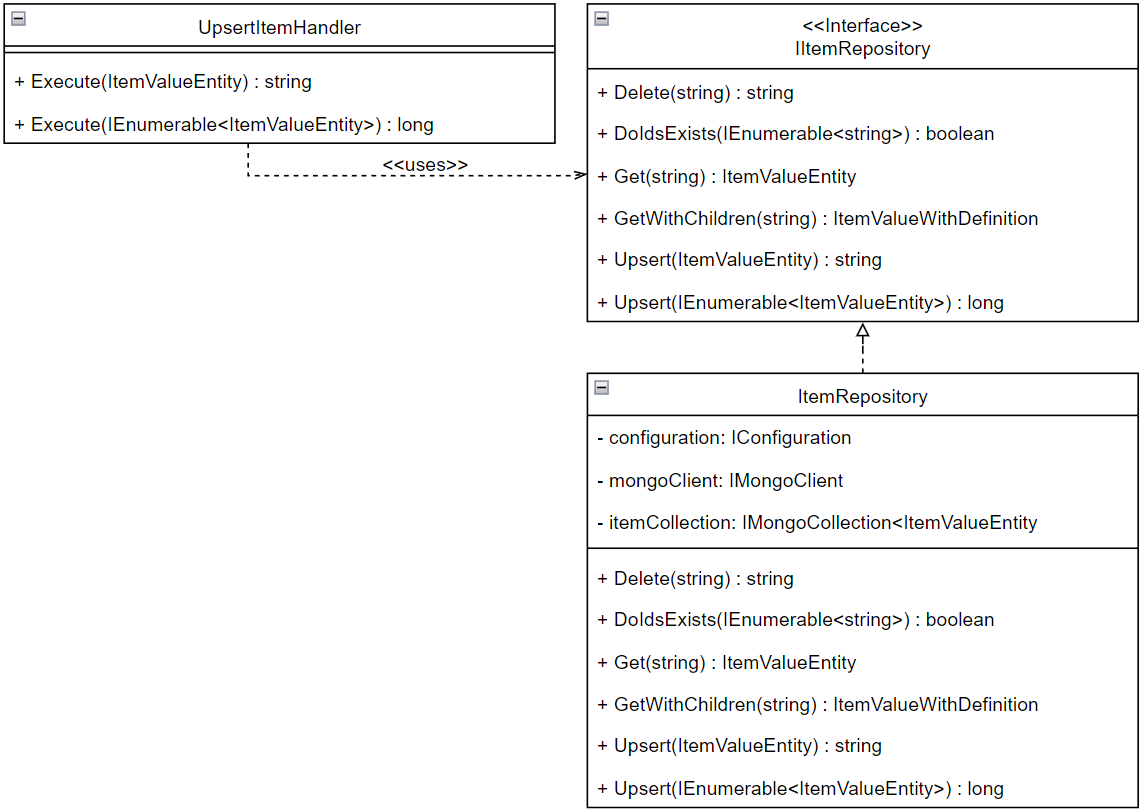
\includegraphics[scale=0.33]{ImplementationRepositoryPatternUML.png}
    \label{fig:RepositoryPatternUML}
\end{graphic}
